\documentclass[conference]{IEEEtran}
%\usepackage{cite}
\usepackage[pdftex]{graphicx}
\usepackage[cmex10]{amsmath}
\interdisplaylinepenalty=2500
\usepackage{algorithmic}
\usepackage{array}
\usepackage{mdwmath}
\usepackage{mdwtab}
\usepackage{eqparbox}
\usepackage[caption=false,font=footnotesize]{subfig}
\usepackage{fixltx2e}
%\usepackage{stfloats}
\usepackage{url}
\hyphenation{op-tical net-works semi-conduc-tor}

% additional packages and utility commands
\usepackage{color}

\newcommand{\TODO}{\textbf{\color{red}TODO}}

\begin{document}

\title{Lowering the Impact of Intrusion Detection\\
on Resources in Wireless Sensor Networks\\
using Code Generation Techniques}

\author{\IEEEauthorblockN{Christophe Van Ginneken, Jef Maerien, Christophe
Huygens, Danny Hughes, Wouter Joosen}%
\IEEEauthorblockA{iMinds - DistriNet - KULeuven\\
B-3001, Leuven, Belgium\\
Christophe.VanGinneken@student.kuleuven.be,\{firstname.lastname\}@cs.kuleuven.be}}

\maketitle

\begin{abstract}
  
Introducing intrusion detection in wireless sensor networks proofs to be a
battle for resources. Implementing and optimizing a collection of detection
algorithms to match the available resources without augmenting the production
costs beyond proportion, might very well be an unacceptable economic burden.
This paper introduces a domain specific language to formally describe such
algorithms and proposes the use of code generation techniques to automate the
production of detection software. This automated process allows for the
optimization of resource usage, more specifically the optimization of the
execution of algorithms and the use of the energy-costly wireless radio. A
prototype code generator was constructed to show that these techniques can be
implemented effectively, resulting in a combination of different intrusion
detection algorithms with less impact on the resources than the sum of the
impact of each algorithm by itself.

\end{abstract}

\section{Introduction}

Wireless sensor networks (WSN) are constructed using large numbers of
autonomous embedded devices, called nodes or motes, referring to their
dust-like properties. Their autonomy is rather absolute, being most of the time
battery-powered and deployed in open terrain. Examples of WSN include
monitoring systems in volcanic regions or flood areas. Preliminary successes
have now even steered researchers towards the introduction of WSN in cities and
homes, thus creating smart cities \cite{schaffers2011smart} and smart homes
\cite{chan2008review}.

Due to their involvement in more and more personal applications, securing these
nodes should be a priority. When we entrust these autonomous systems with some
of our most intimate information, for exameple regarding our health
\cite{stankovic2005wireless}, we would of course like them to be well suited to
protect this information.

Securing WSN, and especially single nodes, is a daunting task
\cite{perrig2004security}. Mostly due to their autonomous nature, nodes are
most of the time physically accessible. With physical access comes a wide range
of physical attacks \cite{becher2006tampering} that are hard to detect, let
alone prevent. Even if the nodes aren't physically accessible, their ways of
communicating with the outside world through various forms of wireless
communication, offer a plethora of possibilities \cite{padmavathi2009survey} to
attack them, ranging from low-level meddling with the routing of packets in the
network, up to the application level.

Securing nodes against intrusions should be a primary objective. But often this
turns out to be impossible and intrusions are sometimes only noticed
post-mortem. When prevention is not guaranteed, a second line of defence
consists in the detection of intrusions, allowing reactive systems to be
introduced to prevent future problematic situations. These intrusion detection
systems (IDS) are well-known in classic networked environments, but are not
easily transferred to the WSN world
\cite{zhang2000intrusion,djenouri2005survey}, mostly due to the wireless and
ad-hoc nature of the networks and the lack of a central point where
communication can be monitored.

But WSN bring even another problem to the table: resources. Due to their vast
deployed numbers and policy to be replaced rather than salvaged, nodes
typically need to be cheap. Their limited functional requirements allow for
them to be built using simple components without redundancy or excess margins.
This introduces an inherent problem for IDS. These systems not only typically
require a lot of resources to store detection information and have to execute
their algorithms over and an over again, but also want to inspect every single
network packets that's passing by. This way they not only would like the node
to be powered-on all the time, they also need constant access to the wireless
radio, which turns out to be the number one energy-consumer of a node.
Introducing IDS in WSN turns out to be a battle for resources.

Finally, besides the technical resources, there is also an economic resource
that plays an important part here. Given the same limited functionality, adding
a complex piece like IDS, might very well augment the production cost well
above acceptable levels. The fact that IDS algorithms are currently in a mere
state of research, would currently require a developer to read through many
research papers, making a selection of algorithms and implement them from
scratch. Even if implementations for each of these algorithms would be
available, the chance that they are applicable to the target platform is
another big if. Integrating these algorithms in itself is already a complex
matter.

Our contribution to IDS in WSN is the introduction of a domain specific
language (DSL) to formally describe IDS algorithms. The DSL is node-oriented
with a strong focus on inter-node communication and aims to allow for the
optimisation of execution of multiple IDS algorithms, thus lowering the
sequential and iterative execution of algorithms and optimizing the use of the
wireless radio.

By introducing such a formal, platform-independent language to express IDS
algorithms and accompanying this language with a code generation framework,
offers an end-to-end solution to many of the problems introduced above:
research output would be directly applicable in a development environment. The
code generation framework allows developers to simply select algorithms and
have platform-specific code without any effort. Due to the possibility to
optimize the use of resources, the impact of introducing IDS on resources in
WSN can be lowered to such extend that more algorithms can be added, thus
augmenting the barriers for intruders, which can help to reduce the number of
successful intrusions.

The remainder of this paper proceeds as follows: section \ref{section:related}
introduces the field of IDS in WSN by means of several IDS algorithms from
research papers. Section \ref{section:problem} describes the problem space in
detail, covering the different parties involved and their contributions.
Section \ref{section:solution} introduces our proposed overall solution, which
is further detailed in sections \ref{section:foo-lang} and
\ref{section:prototype}, which respectively present our domain specific
language, FOO-lang, focusing on the optimization of the organization of
functionality, as well as a prototype implementation of a code generator
framework to complement the language. Section \ref{section:evaluation}
evaluates the prototype implementation and determines if the theoretical merits
of introducing FOO-lang, are actually viable. Finally, section
\ref{section:conclusions} presents our conclusions and proposes topics for
future research to fine-tune the initial findings.

\section{Related Work}
\label{section:related}

Securing any network initially tries to prevent intrusions from happening. This
should of course be a primary concern. But not all intrusions can be prevented
and we need to fall back to detecting intrusions. In this section we take a
look at recent contributions in this field.

Intrusion, or attacks, on computer networks can take many forms. In the case of
WSN this classification needs to be extended even further. In
\cite{padmavathi2009survey} a good overview of both is presented, showing
clearly that WSN suffer from their wireless-communication and broadcast nature.
This causes many attacks based on e.g. eavesdropping to be nearly impossible to
detect while they are happening. Only when the actual intrusions, based on
collected information, have happened, the intrusion could possibly be detected
given the after-effects. This means that we can't cover the entire spectrum and
need to focus on what is feasible.

Research into IDS in WSN typically focuses around two major topics that
complement the architecture of WSN: the nodes as single entities and the
network as a group of such nodes. Both are important because the group cannot
decide without members that detect malicious behavior and a group-based
decision is often needed because nodes can easily miss out on certain events
that could indicate intrusions, due to their wireless and not-always-on nature.

\subsection{Detecting Intrusions}
\label{subsection:detecting}

There are many different ways to construct a taxonomy for intrusion detection,
but common themes do show. According to \cite{mishra2004intrusion} and
\cite{ioannis2007towards} there are three major categories: anomaly detection,
signature or misuse detection, and specification-based detection. In
\cite{alrajeh2013intrusion} the authors agree mostly with this topology, but
add the notion of hybrid intrusion detection systems and cross layer intrusion
detection systems as recent advances in research. Although these additional
categories offer very interesting prospects, the authors have to admit that the
impact on the resource-constrained sensor nodes might still be too high.

The meshed network topology of WSN and its routing protocols has produced many
related attacks and each of these attacks has been the focus of many research
papers presenting algorithms to detect them. In the following paragraphs we
take a look at some of the popular ones.

In a wormhole attack, an artificial low-latency link is created between two
distant nodes in the network. This causes the routing protocol to divert more
traffic through this link, offering the attacker with an abundance of packets
to inspect. In \cite{maheshwari2007detecting} an algorithm is proposed to allow
nodes to determine if a wormhole is actively present. In essence, the algorithm
resides on the exchange of neighbour lists to allow nodes to determine if
unexpected substructures are present in the graph representing the network.

The wormhole attack typically doesn't need to alter any nodes and can make do
with adding two additional nodes in the network. When this addition goes
unnoticed, the wormhole can successfully be constructed. Another attack that is
related to the wormhole is the sinkhole. When launching a sinkhole attack, as
described in \cite{krontiris2008launching}, the attacker first needs to
compromise an existing node. He can achieve this without changing the node's
software and thus control the node in an external way, e.g. using a laptop.
Being in control of the node, the attacker will alter the information provided
to the distributed routing algorithm to make his captured node look
\emph{attractive} to the surrounding nodes and thus draw as much traffic as
possible to itself. The sinkhole attack is typically a foundation for other
routing level attacks, such as selective forwarding, modification of packets or
even dropping them altogether. In its simplest form, the sinkhole offers the
attacker with lots of packets to analyse and use to gather information about
the network and its functionality. Detecting sinkholes is very hard and often
is only possible based on other attacks that are supported by the sinkhole.
When the sinkhole is used to implement selective forwarding,
\cite{ngai2006intruder} proposes an algorithm that allows a base station, the
aggregating master node where all nodes typically send their information to, to
observe missing data from nodes in the same area in a statistical way.

More typical attacks such as flooding, the sybil attack, rushing,\dots are
presented in \cite{wood2002denial} and \cite{djenouri2005survey}.

\subsection{Cooperative Decision Making}
\label{subsection:coorperative}

As in many other situations, a group is often stronger that the sum of its
individual components. This is surely the case for WSN. Because not all nodes
are always actively participating in the network, some nodes might miss queues
that would otherwise lead them to detect intrusions. It is hardly impossible
for a single node to detect a complex attack by itself. Therefore a second
important research topic consists of cooperative algorithms used to combine
information from single nodes into a group-based decision about alleged
intrusions and intruders.

In \cite{krontiris2009cooperative}, the authors first present a theoretical
foundation the analyse cooperative algorithms. Given these foundations they
continue to present an algorithms consisting of 5 phases. It essentially
implements a voting system to identify an intruder based on the Guy Fawkes
protocol \cite{anderson1998new} to exchange suspected intruder information and
allow distributed authentication of those so called votes. Based on these
authenticated votes, a distributed decision can be made about the commonly
identified intruder.

A distributed, cooperative algorithm can sometimes be implemented locally. This
is illustrated by the reputation-based detection algorithm introduced in
\cite{ganeriwal2008reputation}. Using this algorithm, nodes can exchange
information about the reputation of other nodes. Combining this information
allows them to decide about their trust in a given node, using more than only
their own observations.

\subsection{Software Attestation}
\label{subsection:attestation}

A research topic that lives parallel to the detection/cooperation duality is
that of software attestation. Software attestation basically tries to offer
algorithms for exchanging information about the software that is running on a
node, and aims to identify nodes that can no longer prove that their content is
unaltered. Examples of evolving algorithms to implement this functionality
include SWATT \cite{seshadri2004swatt}, ICE/SCUBA \cite{seshadri2006scuba} and
SAKE \cite{seshadri2008sake}. The list of authors shows that this topic lives
strong in certain groups.

Software attestation is hard and many details can cause an algorithm to fail.
Interesting is the discussion surrounding this topic that was started by
\cite{castelluccia2009difficulty}, in response to the previously mentioned
papers. In \cite{perrig2010refutation} the authors of the original papers
counter many of the objections made to their work, but the general feeling is
that even in the best conditions, there is always a backdoor that allows to
circumvent even the most ingenious algorithm to perform software attestation.

\section{Problem Analysis}
\label{section:problem}

The problem of introducing IDS in WSN is much broader than simply the
implementation of a software component. It starts at the very foundations of
WSN. In contrast with for example SNORT \cite{roesch1999snort}, there is
currently no community based collection of algorithms that can be implemented.
The reason is mostly due to the lack of a central/external location where all
network traffic can be analyzed out-of-band. In WSN it's not possible to create
a single entity that will monitor the WSN as is the case in a classic wired
network. Therefore, all algorithms typically evolve independently, without any
cohesion.

Even more, all of these algorithms lack a common, formal notation. In the case
of SNORT, a detection language is provided and new signatures are added on a
regular basis, creating an ever growing rule base, capable of detecting even
the newest of attacks out there.

If implementers of WSN want to add IDS to their network, and therefore to the
nodes in the network, they are facing no small task: first they need to collect
research papers, from which they need to extract the proposed algorithms. Even
if the papers would come with an implementation of their algorithm, the chance
that the implementation matches the target platform of the newly created WSN is
slim.

Simply implementing the different algorithms in sequence, or reusing existing
implementations if they would be available, is also no valid option. All of
these algorithms typically perform the same actions: first they analyze each
incoming packet and collect information about nodes, and secondly at given
intervals, they loop over all known nodes, checking the aggregated information
about them and make decisions about the trust to put in them. While performing
all of these tasks, the algorithms typically also exchange information with
other nodes to complement their own findings.

If such algorithms would be simply combined in a sequential way, the resulting
code would be far from optimal and would consume many of the resources of the
node it runs on: the repetitive parsing of the received packets would result in
much longer processing times than needed, while the chattiness of the
inter-node communication would result the wireless radio being on much more
than wanted.

The cost to implement multiple algorithms over and over again, because due to
the need to optimize the code organisation, would soon outweigh the available
budget of any WSN implementation. If not, the risk to make mistakes in the
sometimes complex algorithms or the lack of flexibility to change sets of
detection algorithms on a regular basis, or simply add a new algorithm in an
easy way, are all very valid reasons to not go down this way. But we still need
to be able to add some form of IDS to WSN.

\section{Proposed Solution}
\label{section:solution}

Different approaches are possible to address the problems identified above. A
major contribution would consist in the creation of a software framework that
accommodated some of the typical usage patterns: a generic payload parser could
be envisaged that allows algorithms to hook in using callbacks, thus making
sure that the parsing is only done once and not repeated for each algorithm.
Secondly, such a framework could collect all outgoing messages and combine them
in a single outgoing packet at the end of a cycle of the node's event loop.

Such a framework comes with guidelines on how to use it, but still relies on
the good behaviour of its users. Also, the integration of the algorithms with
this framework would still be manual work and reconfiguration would typically
impact this part of the implementation. Finally, such a framework does support
the implementation, but still requires thorough analysis of research material
and extraction of the relevant algorithms.

In the case of SNORT \cite{roesch1999snort}, or any other classic network IDS
for that matter, the central detection engine accepts formal descriptions of
signatures of attack patterns. Because it isn't possible to create such a
central component once, there has been no urge to describe detection algorithms
in a formal way. If we now introduce code generation techniques to convert a
formal, platform-independent description of detection algorithms, and generate
this central component, we can bridge the remaining gap.

Code generation allows for the creation of code that implements the actual
algorithm. The algorithm can be described in a platform-independent way,
therefore allowing reuse of the algorithm on multiple platforms. The generated
code can further access a minimal software framework that covers common tasks
and/or platform specific functionality.

Given formal descriptions of the algorithms, a implementer of a new WSN
application could simple select a set of algorithms, feed their formal
description to the code generator and automatically receive platform-specific
code, optimized for execution and communication.

A formal description of detection algorithms would not only be beneficiary to
implementers. Also to researchers such medium would offer substantial benefits.
Formal descriptions of these algorithms not only allows for generation of code,
but the same descriptions can be loaded into simulators and be investigated in
combination with other algorithms \cite{mernik2005and}, formal analysis of the
algorithms would be an interesting option. Further, describing the algorithms
in a platform-independent way, would increase their usefulness and allow for
more complex algorithms to be abstracted.

\section{Introducing FOO-lang}
\label{section:foo-lang}

The central component of our proposed solution is a formal description of
intrusion detection algorithms. This formal description can be realized using a
domain specific language (DSL). Before actually defining a new language, it is
important to ensure that the reasons to do so are legit. Too often languages are
implemented too quickly, where coding conventions or frameworks with well
thought-out API's fit the bill quiet nicely.

The line can not be drawn in a black and white fashion and DSL do have
benefits, but don't come for free \cite{mernik2005and}. Many good reasons why
to implement a DSL, or not, can be found in \cite{van2000domain},
\cite{mernik2005and} and \cite{fowler2010domain}. Based on these, we try to
justify our choice to propose a DSL for this solution.

\subsection{Justification of the Use of a DSL}
\label{subsection:justification}

The primary goal is the proposed solution is to avoid the creation of bad code
that drains the limited resources of a node. Two basic examples are presented
to illustrate this bad behaviour: repetitive execution of the same tasks, such
as parsing or iterating over a set of known nodes and the use of the wireless
radio.

The latter can be covered by a framework, as illustrate earlier. It comes with
an obligation to actually use the framework. One cannot protect users against
their own stupidity if they don't follow the rules. The former is a bit
trickier. Let's say that we would use the C language as a lingua franca to
complement the framework, which hides the platform specific parts. This would
be valid, but offering a complete language would soon result in loops that
break with the guidelines and would undermine the conceptual idea of optimizing
the organisation of the functionality.

Restricting the formal description to a subset that doesn't allow for
constructions that violate the goals, is in this case a valid reason to tend
towards a DSL. Introducing a DSL further also allows for more functional ways
of handling the concepts that are part of the domain. In this case the domain
clearly consists of inter-operation between nodes and local processing of
algorithms that typically deal with sets of nodes. Although that C comes close
to a lingua franca amongst both researchers and implementers, it is still a
very low-level language with very little support for concise operations such as
pattern matching, event-driven-ness,\dots.

If C doesn't fit this profile, maybe another language does. During the early
days of our research, we looked at a language that seems to fit the required
functionality like a glove: Erlang. It comes with strong communication
paradigms, has pattern matching, is event-driven by nature,\dots and according
to \cite{wong1998compiling} it even can be translated to C. This road looked
very promising, but as with any other general purpose language, it was to
capable and would allow for constructions that would thwart the envisaged
optimizations.

\subsection{Design Principles for FOO-lang}
\label{subsection:design}

\TODO

\section{Prototype Code Generator}
\label{section:prototype}

\TODO

\section{Evaluation}
\label{section:evaluation}

\TODO

\section{Conclusions and Future Work}
\label{section:conclusions}

\TODO

\section*{Acknowledgements}
\label{section:acknowledgements}

We would like to thank the reviewers for their thoughtful and helpful comments
that enhanced the readability of this paper. Our gratitude and respect also
goes out to all members of the WSN work group at KU Leuven for creating the
nurturing environment where these ideas could grow.

\bibliographystyle{IEEEtran}
\bibliography{referenties}

\end{document}

% \begin{figure}[!t]
% \centering
% 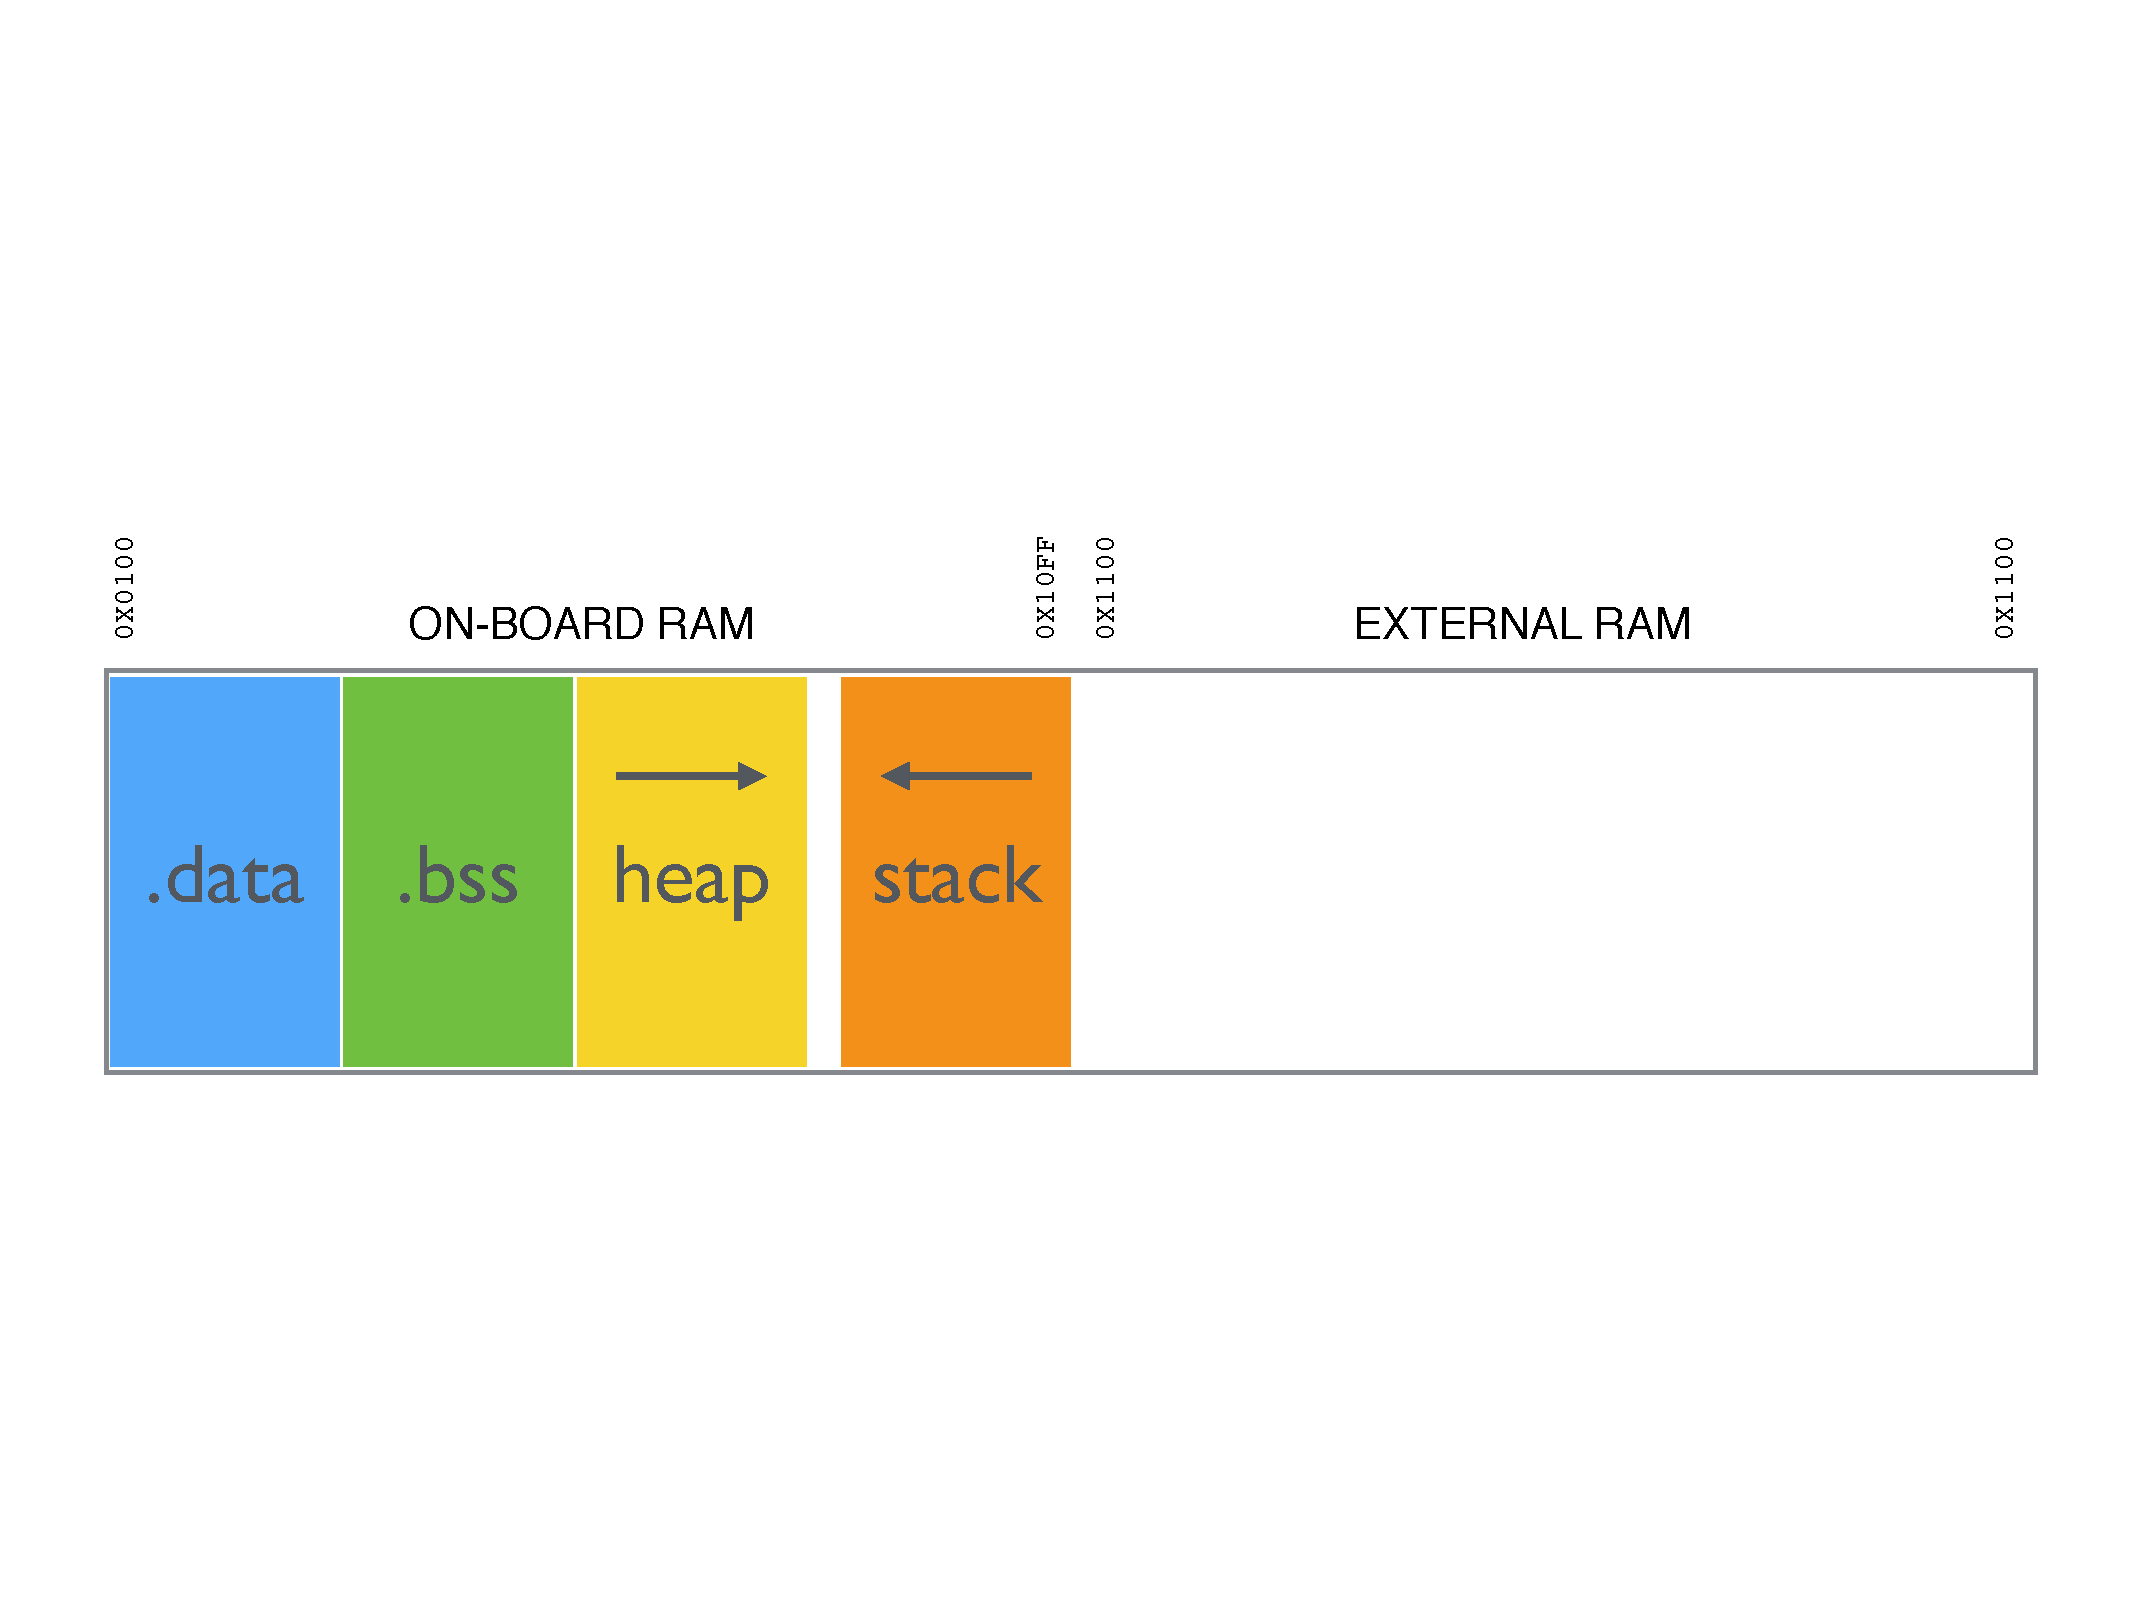
\includegraphics[width=2.5in]{resources/avr-ram-map.pdf}
% \caption{Simulation Results}
% \label{fig_sim1}
% \end{figure}
% 
% \begin{figure*}[H]
% \centering
% \subfloat[]{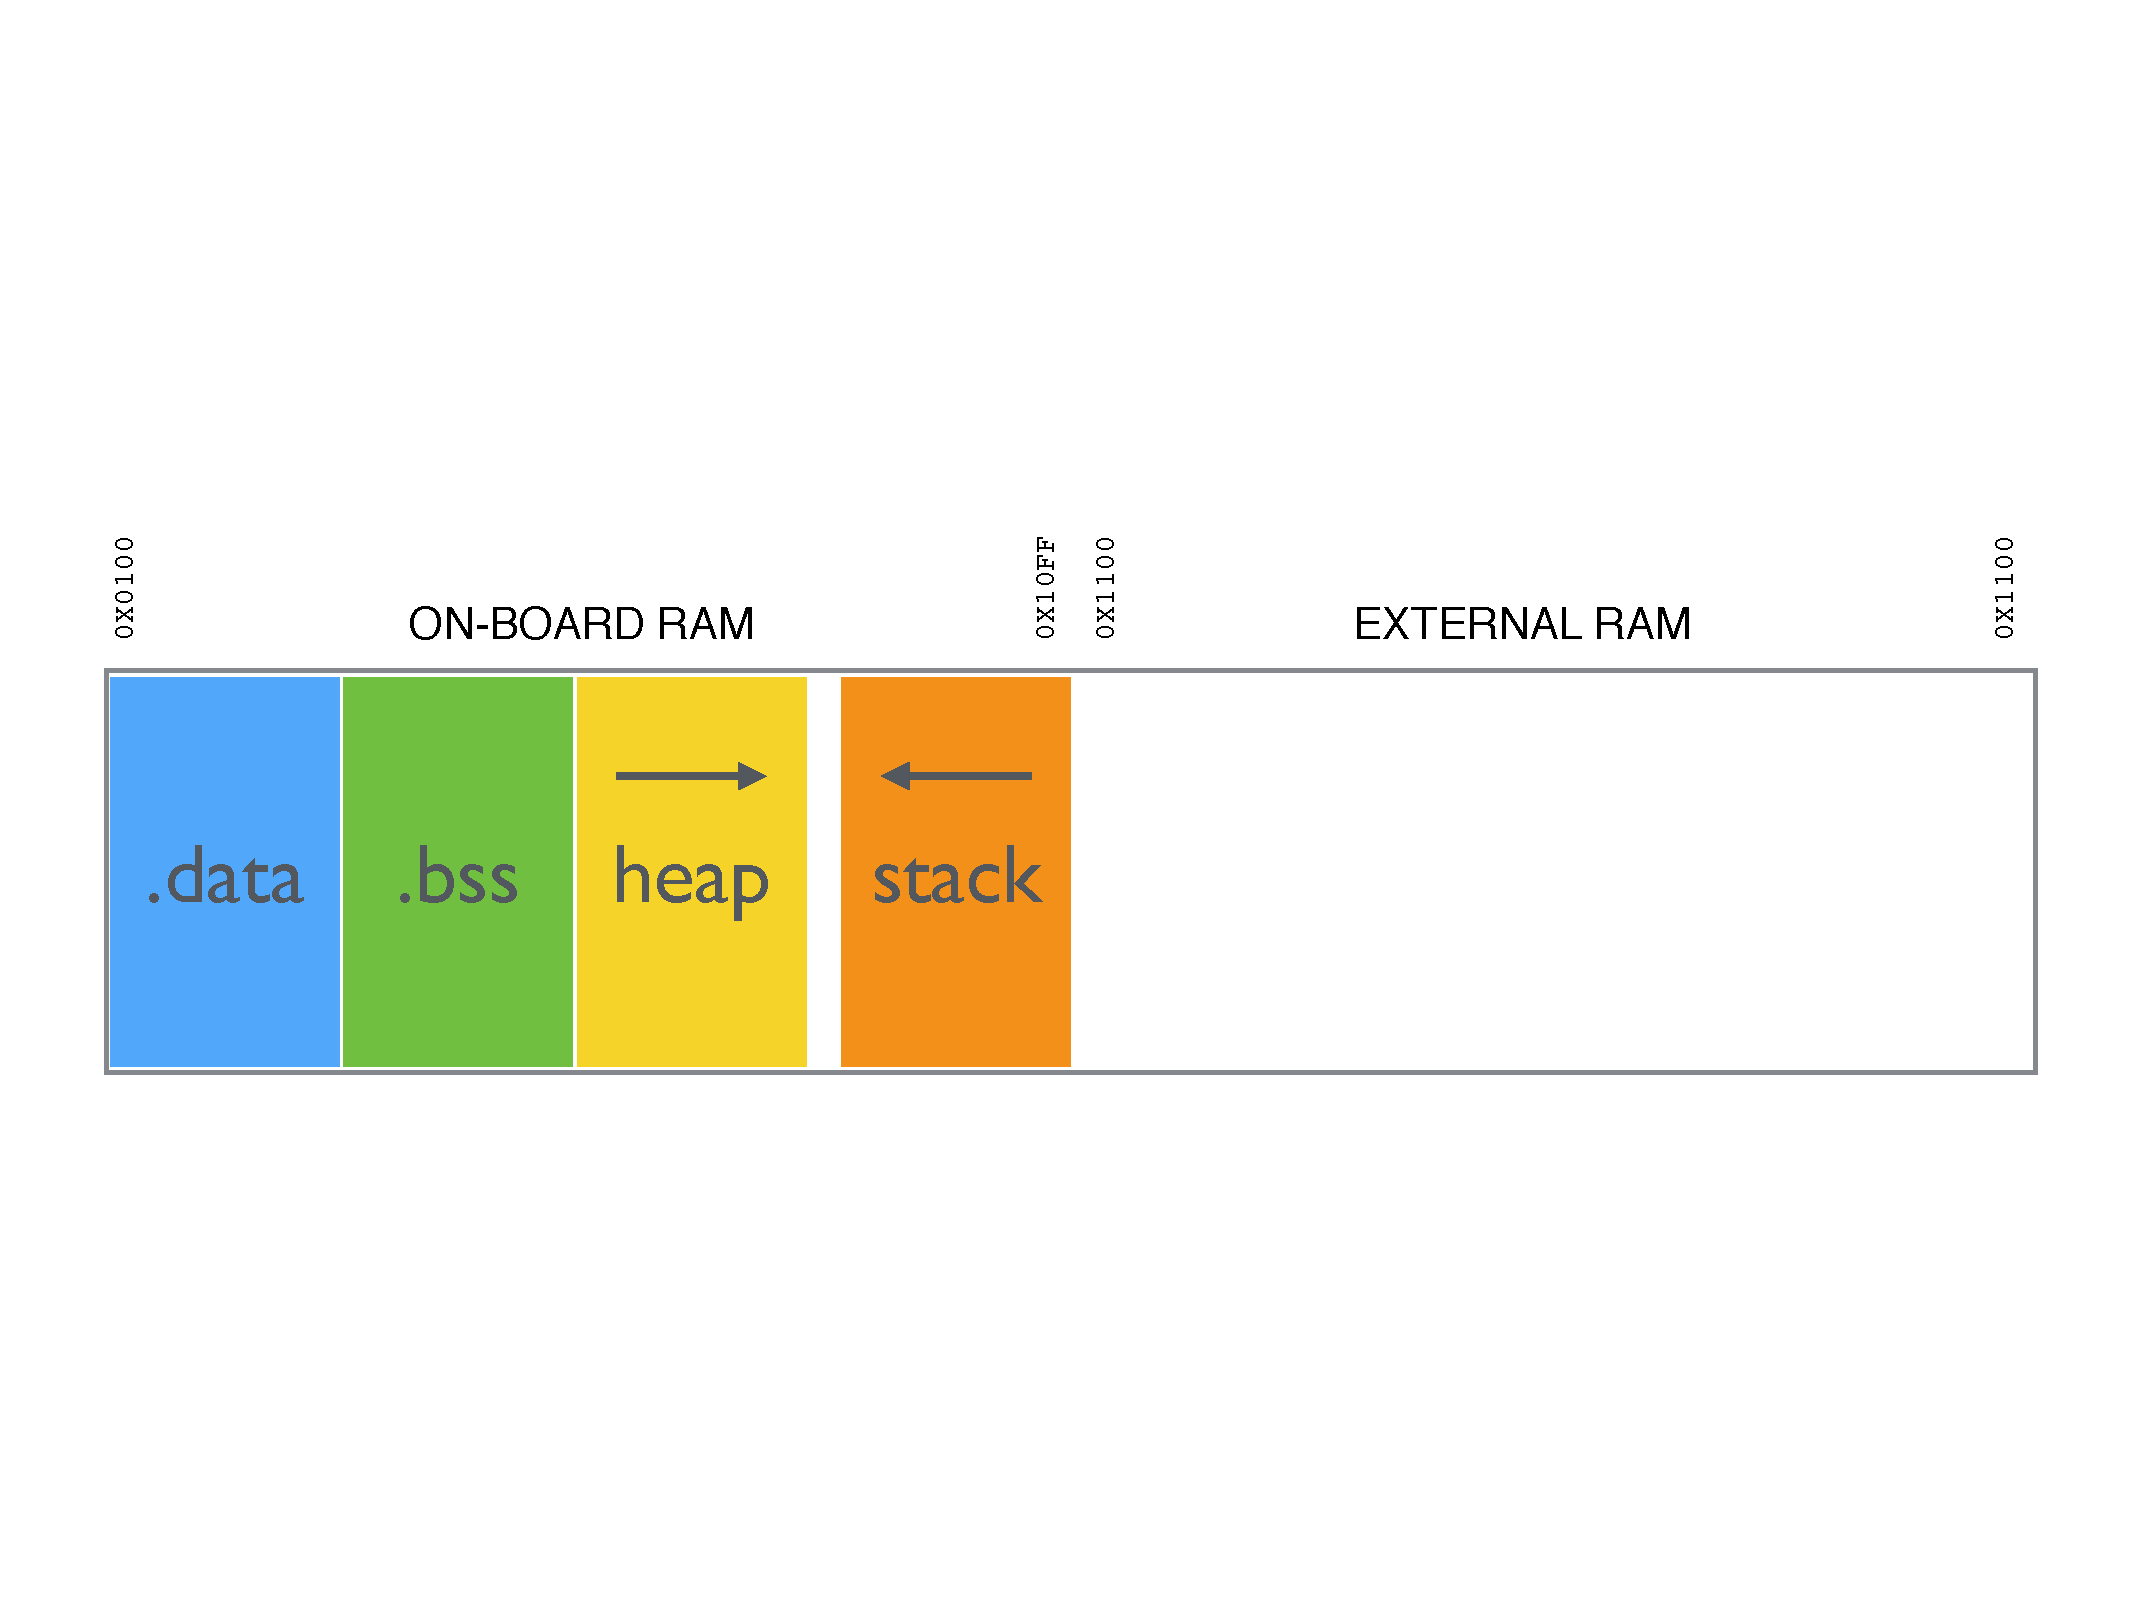
\includegraphics[width=2.5in]{resources/avr-ram-map.pdf}%
% \label{fig_first_case}}
% \hfil
% \subfloat[]{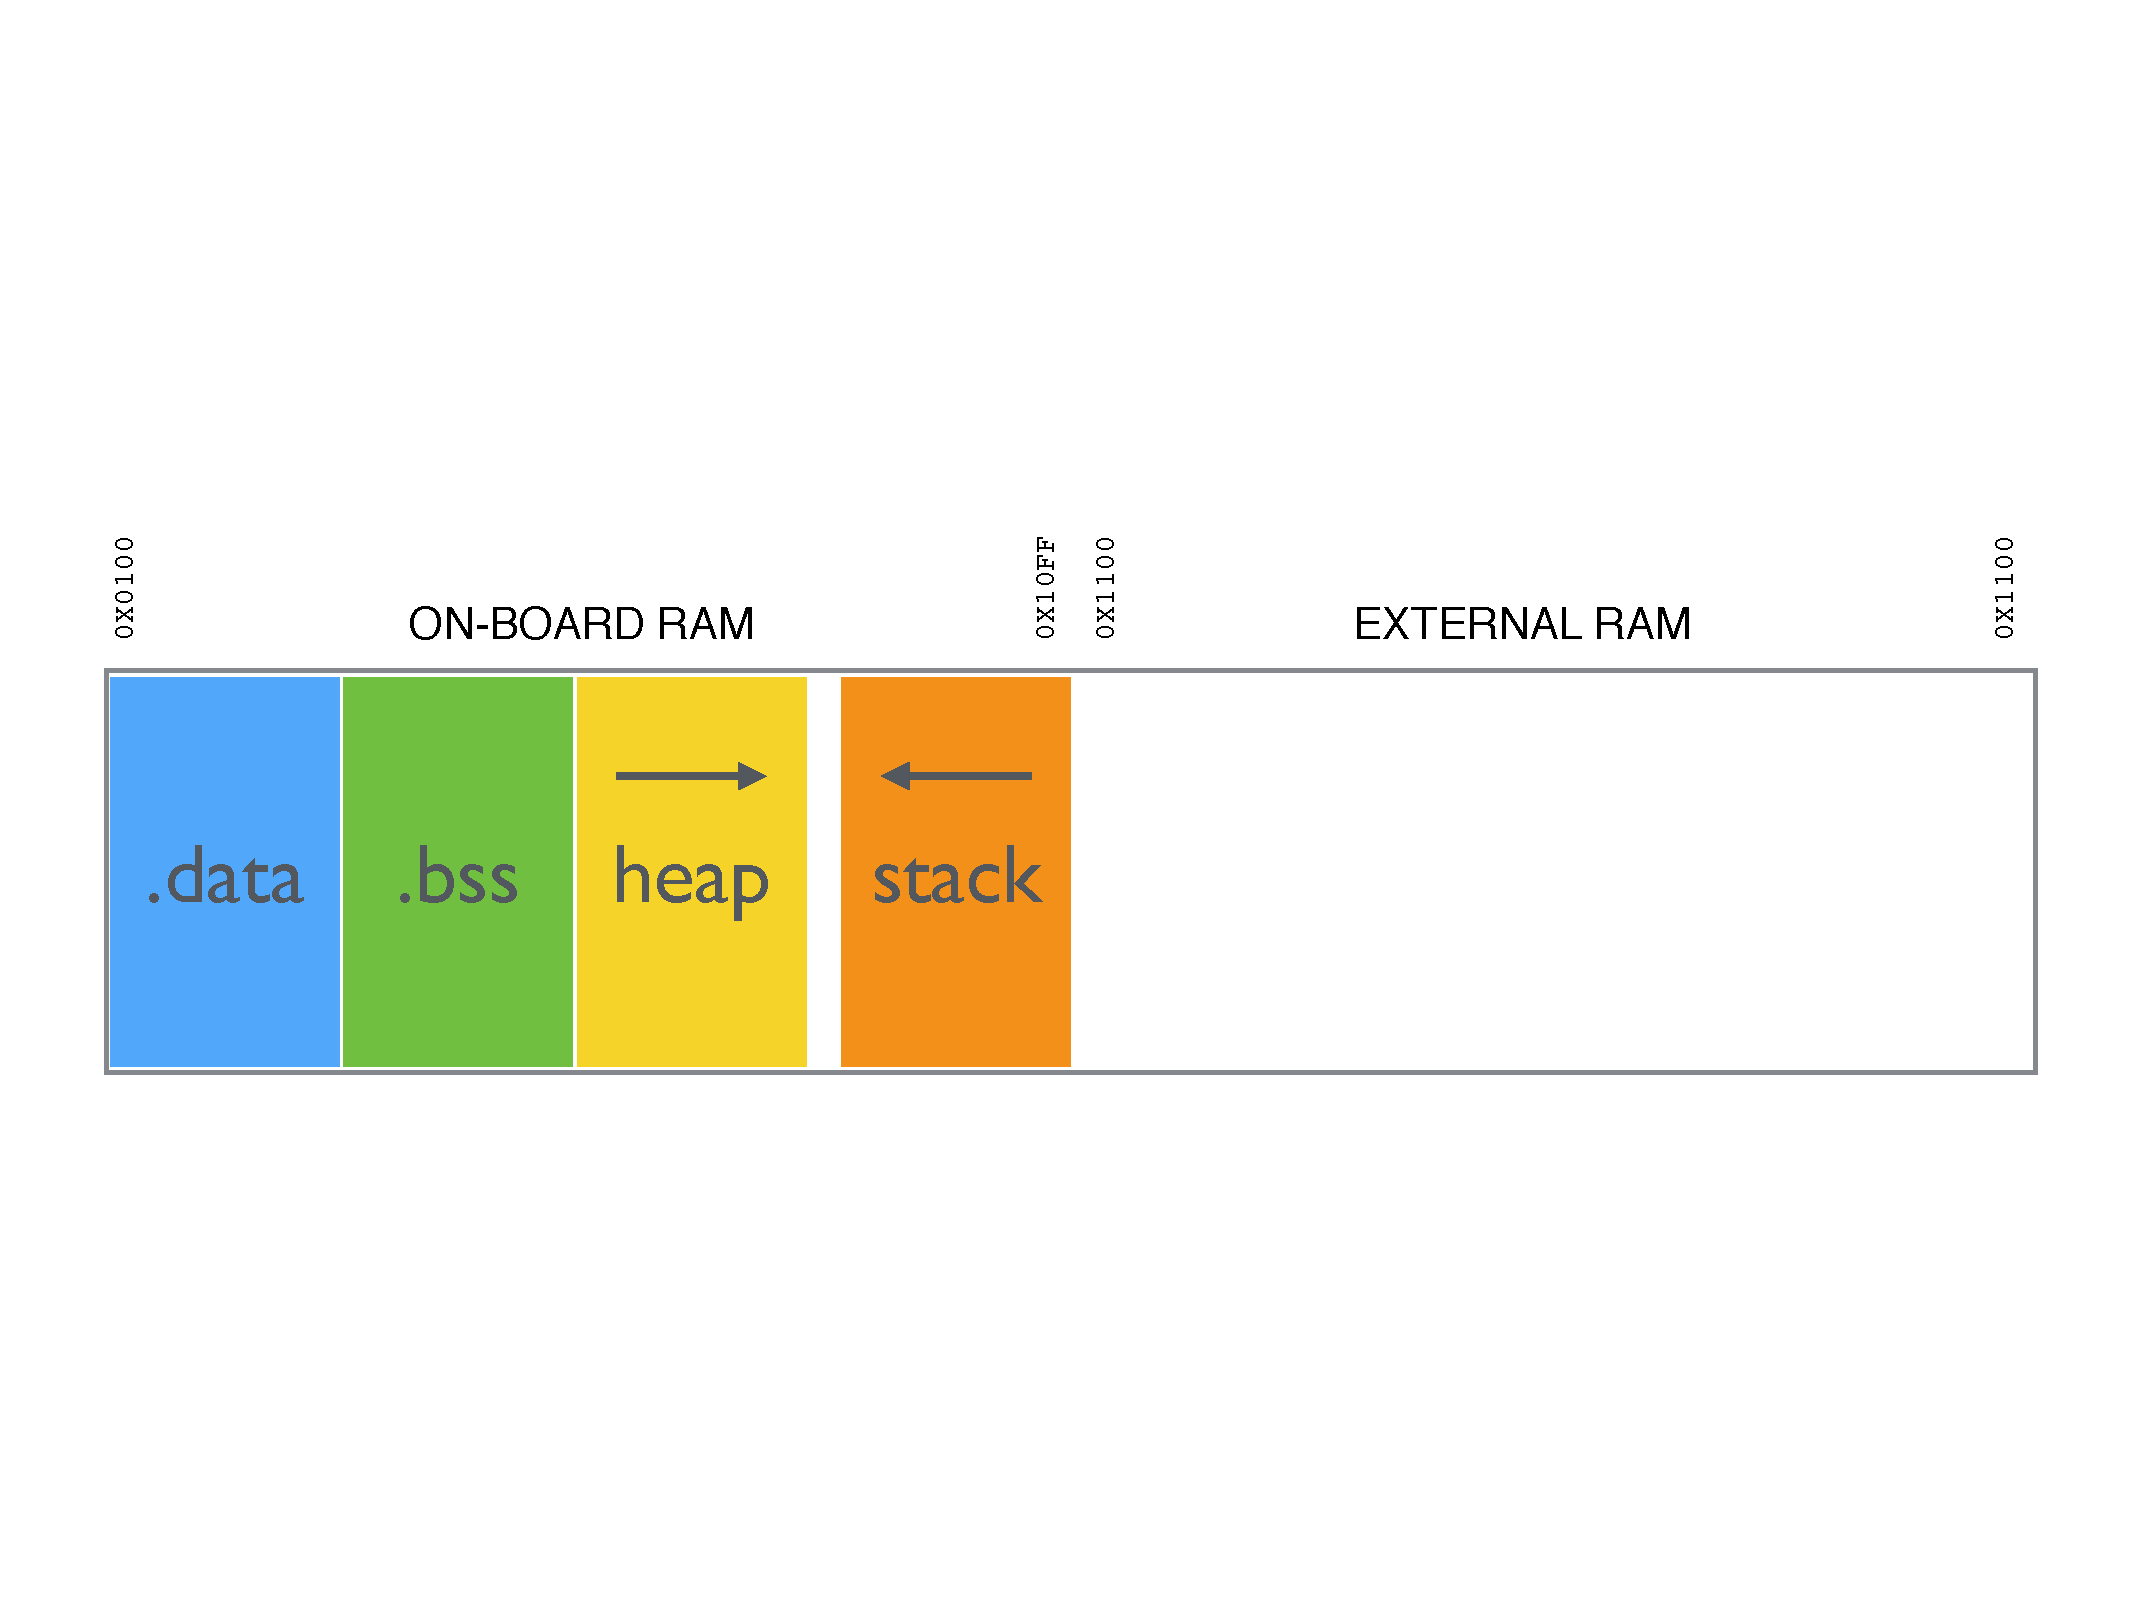
\includegraphics[width=2.5in]{resources/avr-ram-map.pdf}%
% \label{fig_second_case}}
% \caption{Simulation results: (a) Case I (b) Case II}
% \label{fig_sim2}
% \end{figure*}
% 
% \begin{table}[!t]
% \renewcommand{\arraystretch}{1.3}
% \caption{An Example of a Table}
% \label{table_example}
% \centering
% \begin{tabular}{|c||c|}
% \hline
% One & Two\\
% \hline
% Three & Four\\
% \hline
% \end{tabular}
% \end{table}


